\chapter{Servidor}
% Java - REST - JSON - JSOUP 

Com o objetivo de extrair e preparar as informações a serem consumidas pela aplicação móvel do sistema acadêmico Minha Uno, foi desenvolvido em linguagem Java um servidor REST para facilitar e agilizar a extração dos dados. 

Como no questionário apresentado anteriormente obtemos maior quantidade de respostas referentes aos acadêmicos de cursos de graduação, então para este trabalho foi escolhido implementar o servidor e posteriormente a aplicação para este público alvo, sendo implementados os módulos que apresentaram as três melhores notas, sendo eles Material de Apoio, Notas da Graduação e Horários do Semestre.

Utilizando-se da biblioteca \emph{jsoup} para a extração das informações e após o tratamento dos dados gerando-se arquivos JSON transmitidos utilizando um servidor REST, serão detalhadas nas próximas sessões o funcionamento de cada etapa da extração, preparação e transmissão das informações desde o sistema acadêmico Minha Uno até a aplicação móvel.

\section{Ferramentas Utilizadas}
Para o desenvolvimento do servidor foram utilizadas apenas ferramentas Open-Source, sendo que a linguagem escolhida para o desenvolvimento foi o Java, devido a quantidade de documentação encontrada na internet, e também por possuir bibliotecas prontas que permitem a extração, tratamento e disponibilidade das informações, facilitando assim a implementação do servidor.

\section{Extração das Informações}

Segundo informações obtidas da diretoria de Ti da Unochapecó, a instituição não possui um webservice com as informações do sistema acadêmico, e desta forma as informações exibidas na página são extraidas diretamente de uma coleção de banco de dados, o que tornaria inviável a integração direta com estas bases. Com a excasses de alternativas, foi necessário extrair as informações diretamente da página do sistema acadêmico. Para todos os processos de extração foi utilizada a biblioteca \emph{jsoup}, sendo que a mesma é responsável pela conexão aos diferentes endereços do sistema acadêmico e pela extração das informações a partir do retorno das consultas de navegação, ou seja, sendo extraidas as informações a partir do HTML retornado pelo sistema acadêmico atual.

Após o devido tratamento utilizando-se filtros com expressão regular e outros comandos permitidos pelo \emph{jsoup}, as informações necessárias para a aplicação são obtidas, sendo que na continuidade do capítulo será explicado como cada grupo de informações foi extraido e posteriormente preparado para ser consumido pelos dispositivos móveis.

Todas as expressões utilizadas na biblioteca \emph{jsoup} podem ser testadas na página web \url{http://try.jsoup.org/} utilizando como entrada o código HTML da página a ser analizada. Mais informações sobre as expressões utilizadas podem ser obtidas em \url{http://jsoup.org/cookbook/extracting-data/selector-syntax}.

Como toda a extração é baseada no retorno do código HTML do sistema atual, qualquer alteração no layout do arquivo HTML retornado pela página do sistema acadêmico Minha Uno resultará em problemas na extração dos dados.


\subsection{Login}
Com o objetivo de validar se o login fornecido pelo usuário na aplicação é válido e extrair o cookie (identificador de sessão utilizado para as acesso as informações obtidas apenas pelo login válido do usuário), o servidor possuí como primeira tarefa ao receber uma solicitação da aplicação a validação de login.

Utilizando-se do método POST do HTTP, os dados de login são enviados utilizando o endereço \url{https://www.unochapeco.edu.br/usuarios/login?login_submited=1&usuario=USUARIO&senha=SENHA&submit=entrar} (as palavras USUARIO e SENHA devem ser substituidas pelas respectivas informações).

\begin{algorithm}
\caption{Algoritmo para Validação do Login e Captura da Sessão}
\label{alg:frw}
\algsetup{indent=3em, linenodelimiter=.}
\begin{algorithmic}[1]
\REQUIRE Login e Senha do Usuário
\ENSURE Resultado se as informações de login são válidas e Cookie de Sessão

\STATE var $session$
\STATE var $loginValido$

\STATE var $retornoServidor \gets Resultado da Consulta ao Servidor Minha Uno$
\STATE $sessao \gets retornoServidor.cookie("PHPSESSID")$
\IF{$retornoServidor = InformacaoValidaDeLogin$}
    \STATE $loginValido \gets VERDADEIRO$
\ELSE
   \STATE $loginValido \gets FALSO$
\ENDIF

\RETURN loginValido
\end{algorithmic}
\end{algorithm}

O algoritmo de extração do cookie e validação do login não apresenta nenhuma complexidade, conforme pode-se observar no Algoritmo 1. Para a exemplificação dos algoritmos neste capítulo não será adicionado código fonte em java, exibindo-se trechos de pseudo-código com relevância para este trabalho.

%%% Aqui é a sessão de extração do material de apoio
\subsection{Material de Apoio}
Com o objetivo de extrair a relação dos materiais eletrônicos postados pelos professores em cada disciplina cursada pelo acadêmico. Para melhor entendimento, o algoritmo será dividido em duas partes, sendo que a primeira parte mostrará como são extraidas as informações referentes as disciplinas cursadas pelo acadêmico, e a segunda parte do como são extraidas as informações dos materiais disponíveis.

%O Algoritmo 2 mostra como as informações dos materiais de apoio são extraidas, e o mesmo será detalhado nos itens 5.2.2.1 e 5.2.2.2 deste trabalho.

%%% Aqui é a subsubsessão de extração das disciplinas
\subsubsection{Extração das Disciplinas}
Com o objetivo de extrair a lista das disciplinas pertencentes ao módulo de material de apoio do sistema acadêmico, é necessário que a informação seja extraida a partir do código HTML retornado pela url \url{https://www.unochapeco.edu.br/saa/materialApoio.php}. Para a obtenção das disciplinas corretas cursadas pelo acadêmico, é utilizado o cookie de sessão capturado no momento do login, conforme explicado no item 5.2.1 deste trabalho. Um exemplo de código HTML retornado pelo servidor a partir deste tipo de consulta pode ser visto na url \url{https://gist.github.com/ajzuse/5703254/raw/2257edf4b1b7fb53cec0d5705ae454a5910217ff/materialapoio.html}.

A partir do código HTML retornado, sendo aplicanda a expressão ``\emph{form tr td:eq(1) a}'' sob o mesmo por meio da biblioteca \emph{jsoup}, obtém-se como retorno a lista das disciplinas cursadas pelo acadêmico, conforme pode ser visto na figura 5.

\begin{figure}[!htb]
     \centering
     \caption[Extração de Informações - Lista de Disciplinas do Material de Apoio]{Lista das disciplinas extraidas.}
     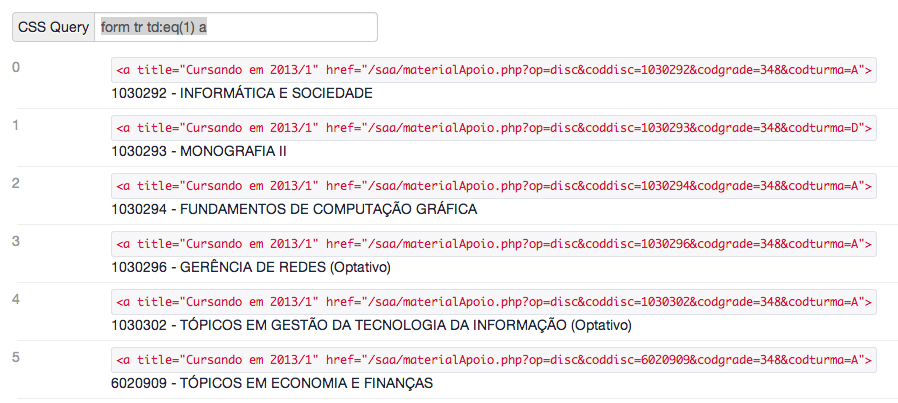
\includegraphics[scale=0.5]{imagens/listadisciplinasmaterialapoio.png}
     \\ Fonte: Do Autor.
\end{figure}

A partir da lista retornada acima, é possível retornar diretamente a disciplina no formato ``\emph{Código - Nome}''. Também como pode-se verificar na Imagem 5, acima do nome da disciplina é exibida a tag HTML completa, sendo que nesta tag pode-se verificar o atributo \emph{href}, que possui o caminho completo para serem extraidos os materiais da disciplina.

Após a extração do nome da disciplina e da tag \emph{href}, é necessária a extração das informações dos materiais da disciplina, explicada na sessão 5.2.2.2 deste trabalho.

%%% Aqui é a subsubsessão de extração dos materiais
\subsubsection{Extração dos Materiais}
Após a extração da lista de disciplinas e da referência ao endereço web onde as disciplinas podem ser acessadas, é necessário extrair as informações dos materiais propriamente ditos.

A partir do código HTML (disponível na url \url{https://gist.github.com/ajzuse/5703254/raw/1c124c120578cabda1dab410077cad5bb867ebbc/listamateriais.html}, sendo que o mesmo é pertencente a uma disciplina do 9º período de Ciência da Computação na grade 348) obtido pela url capturada (conforme explicado na sessão 5.2.2.1). No código retornado, existem 4 informações relevantes, sendo elas: nome, url, publicação e descrição.

Para a extração do nome do material, a expressão ``\emph{form tr:contains(Arquivo) a}'', sendo que a mesma retorna uma lista com o nome das disciplinas, conforme pode ser visto na Figura 6.

\begin{figure}[!htb]
     \centering
     \caption[Extração de Informações - Lista de Nomes dos Materiais de uma disciplina]{Lista de nomes dos materiais de uma disciplina.}
     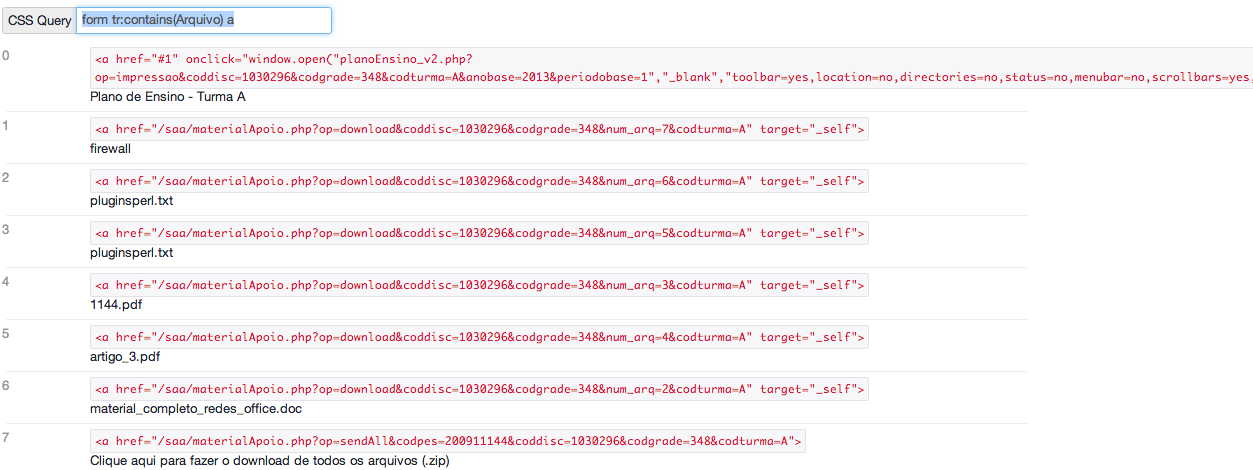
\includegraphics[scale=0.35]{imagens/listamateriaisdisciplinasnomematerial.png}
     \\  Fonte: Do Autor.
\end{figure}

Verificamos na Figura 6 que a mesma expressão retorna no campo principal o nome das disciplinas, e na sua referência (exibida em vermelho) o campo href, que nos é interessante para o acesso direto ao arquivo listado. Desta forma, utilizando-se da mesma expressão é possível extrair a url de acesso direto ao arquivo e também o nome do arquivo a ser acessado. Desta forma, duas informações já são preenchidas a partir da mesma consulta. 

Para obtermos a publicação, que nada mais é o nome do professor que postou o material e a data de postagem, utiliza-se a expressão ``\emph{form tr:contains(Publicação) td:eq(1)}'', e o seu retorno pode ser verificado na Figura 7.

\begin{figure}[!htb]
     \centering     
     \caption[Extração de Informações - Lista das publicações dos materiais]{Lista de publicação dos materiais de uma disciplina.}
     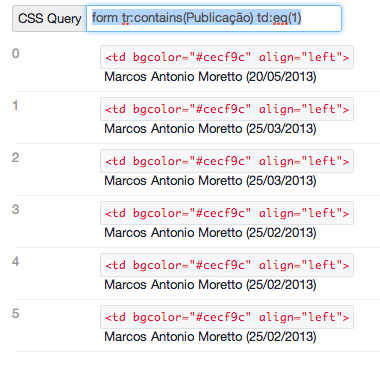
\includegraphics[scale=0.7]{imagens/listamateriaisdisciplinaspublicacao.png}
     \\  Fonte: Do Autor.
\end{figure}

Para obtermos a descrição dos materiais postados, a expressão ``\emph{form tr:contains(Descrição) td:eq(1)}'' onde obtém-se como resultado a lista da descrições dos materiais, confome pode ser visto na Figura 8.

\begin{figure}[!htb]
     \centering
     \caption[Extração de Informações - Lista das descrições dos materiais]{Lista de descrição dos materiais de uma disciplina.}
     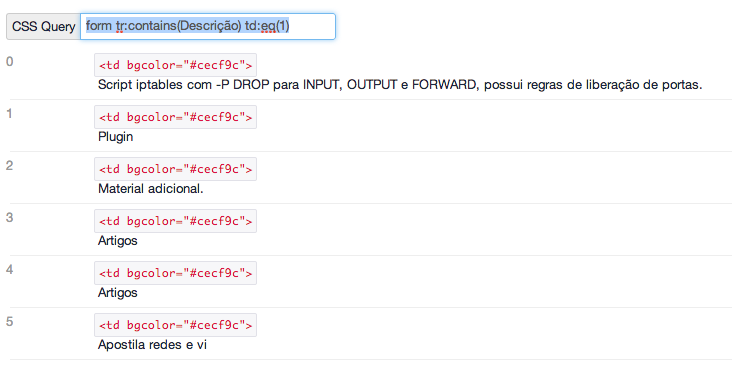
\includegraphics[scale=0.6]{imagens/listamateriaisdisciplinasdescricao.png}
     \\  Fonte: Do Autor.
\end{figure}

\newpage

\subsection{Notas da Graduação}
Com o objetivo de de extrair as avaliações e as respectivas notas das avaliações aplicadas aos acadêmicos, foi desenvolvida a classe de extração das notas da graduação. Para melhor entendimento, o algoritmo será dividido em três partes, onde a primeira representará a extração da lista de disciplinas cursadas pelos acadêmicos, a segunda as informações referentes as avaliações e notas das disciplinas em aberto e a terceira parte explicará a extração das disciplinas já finalizadas pelo acadêmico.

Assim como na sessão 5.2.2, será utilizada a biblioteca \emph{jsoup} para extração das informações, utilizando-se das mesmas recomendações da sessão mencionada anteriormente.

\subsubsection{Extração das Disciplinas}
Com o objetivo de extrair a lista das disciplinas pertencentes ao módulo de notas da graduação do sistema acadêmico, é necessário que a informação seja extraida a partir do código HTML retornado pela url \url{https://www.unochapeco.edu.br/saa/notas.php}. Para a obtenção das disciplinas corretas cursadas pelo acadêmico, é utilizado o cookie de sessão capturado no momento do login, conforme explicado no item 5.2.1 deste trabalho. Um exemplo de código HTML retornado pelo servidor a partir deste tipo de consulta pode ser visto na url \url{https://gist.github.com/ajzuse/5703254/raw/09fc387296dbe312ed7ec9232ddde838b20943fb/notasgraduacao.html}.

A partir do código HTML retornado, sendo aplicanda a expressão ``\emph{form table:eq(0) tr td:eq(1) a}'' sob o mesmo por meio da biblioteca \emph{jsoup}, obtém-se como retorno a lista das disciplinas cursadas pelo acadêmico, conforme pode ser visto na figura 9.

\begin{figure}[!htb]
     \centering
     \caption[Extração de Informações - Lista das disciplinas Notas da Graduação]{Lista das disciplinas das Notas da Graduação.}
     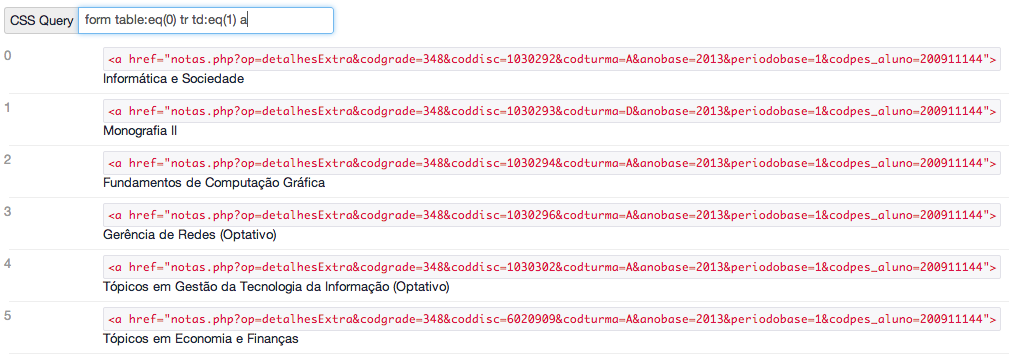
\includegraphics[scale=0.45]{imagens/listadisciplinasnotasgraduacao.png}
     \\  Fonte: Do Autor.
\end{figure}

Como pode ser percebido na Figura 9, além do nome das disciplinas, na parte em vermelho que representa a tag HTML possui o atributo \emph{href}, sendo que o mesmo armazena o link para acesso as avaliações e notas da disciplina em específico, sendo este atributo importante para a a extração das notas e avaliações das disciplinas em aberto, sendo então necessário coletar o mesmo juntamente com o nome da disciplina. Após a extração do nome das disciplinas e da respectiva url a partir do atributo \emph{href}, é iniciada a extração das avaliações por disciplina.

\subsubsection{Extração das Notas e Avaliações das Disciplinas em Aberto}
Após a extração do nome das disciplinas cursadas pelo acadêmico e da url utilizada para acesso a disciplina específica, esta mesma url é utilizada para a extração das avaliações e notas do acadêmico, assim como também das médias do graduando. Para esta extração são utilizadas várias combinações de expressões. Um exemplo de código retornado pode ser consultado na url \url{https://gist.github.com/ajzuse/5703254/raw/95df1ccd4a07589b60859044562450b986e314de/avaliacoes.html}.

Para a extração da lista de avaliações, é utilizada a expressão \emph{form table:eq(0) tr:gt(4)} como base da extração, e posteriormente são aplicadas novas expressões sobre os resultados obtidos da aplicação da expressão base. A Figura 10 nos mostra parcialmente o retorno da expressão.

\begin{figure}[!htb]
     \centering
     \caption[Extração de Informações - Resultado parcial Avaliações]{Resultado parcial da Expressão base sobre as avaliações.}
     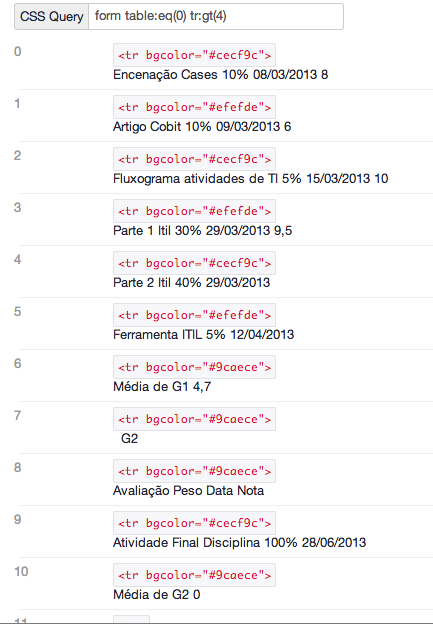
\includegraphics[scale=0.5]{imagens/avaliacoesdisciplinas1.png}
     \\  Fonte: Do Autor.
\end{figure}

Como pode ser percebido na Figura 10, as informações aparecem um pouco misturadas, sendo necessário tratar via programação as informações que realmente serão extraidas e ignorando as informações que não são necessárias. Isto é feito por meio de uma verificação de quando a informação contida na quarta coluna da tabela retornada esta em branco ou contém a palavra notas.

%\textbf{AQUI VAI O ALGORITMO DE EXTRAÇAO DAS AVALIAÇOES E NOTAS DAS DISCIPLINAS!!!!!!}

A partir do retorno acima, são extraidas as seguintes informações das avaliações: nome, peso, data e nota. Cada uma destas informações possui uma expressão aplicada sobre a expressão base. A Tabela 7 contém a expressão para cada informação e a ser extraida.

\begin{table}[!hbt]
\centering
\caption[Extração de Informações - Expressões de Extração]{Tabela de expressões de extração das informações das avaliações}
\vspace{3mm}
\begin{tabular}{p{3cm}|c}\hline
\bf{Informação} & \bf{Expressão} \\ \hline
Nome & td:eq(0)\\ \hline
Peso & td:eq(1)\\ \hline
Data & td:eq(2)\\ \hline
Nota & td:eq(3)\\ \hline
\end{tabular}
\\ Fonte: elaboração do autor.
\end{table}

Para a extração das médias de G1 e de G2 dos graduandos, são utilizadas as expressões contidas na Tabela 8, sendo que estas expressões são aplicadas diretamente sobre o código HTML, não mais sobre a expressão base.

\begin{table}[!hbt]
\centering
\caption[Extração de Informações - Extração das Médias]{Tabela de expressões de extração das médias de G1 e de G2}
\vspace{3mm}
\begin{tabular}{p{3cm}|c}\hline
\bf{Informação} & \bf{Expressão} \\ \hline
Média de G1 & form table:eq(0) tr:contains(Média de G1) td:eq(1)\\ \hline
Média de G2 & form table:eq(0) tr:contains(Média de G2) td:eq(1)\\ \hline
\end{tabular}
\\ Fonte: elaboração do autor.
\end{table}

Após estes procedimentos a extração das avaliações, assim como das médias de G1 e G2 estão concluídas, faltando apenas a extração das notas para as disciplinas já finalizadas pelo acadêmico no semestre.

\subsubsection{Extração das Notas das Disciplilas Finalizadas}
Finalizando a sessão de extração das notas da graduação, a extração das notas das disciplinas já finalizadas ocorre em cima do mesmo código HTML obtido no item 5.2.3.1 deste trabalho, que pode ser consultado na url \url{https://gist.github.com/ajzuse/5703254/raw/09fc387296dbe312ed7ec9232ddde838b20943fb/notasgraduacao.html}.

Devido a ordem em que as disciplinas são exibididas na lista de disciplinas ser diferente a ordem exibida nas notas oficiais da graduação, a expressão utilizada para a busca das notas de disciplinas já finalizadas leva em consideração o código da disciplina encerrada, extraindo o mesmo a partir do atributo href da tag html retornada na lista de disciplinas. Para o retorno das informações da disciplina já finalizada, é utilizada a expressão \emph{form[name\$=graduacao] tr:contains(CODIGODISCIPLINA)}, sendo que a palavra CODIGODISCIPLINA deve ser substituida pelo código propriamente dito.

\subsection{Horários do Semestre}
Com o objetivo de extrair o horário das disciplinas cursadas pelo acadêmico, e também as informações detalhadas da disciplina, foi desenvolvida a classe de extração dos horários do semestre. Para facilitar o entendimento, a explicação do processo será dividido em três partes, sendo elas: Extração do nome das disciplinas, Extração das informações gerais da disciplina e Extração dos Horários de Aula.

\subsubsection{Extração das Disciplinas}
Com o objetivo de extrair a lista das disciplinas pertencentes ao módulo de horários do semestre do sistema acadêmico, é necessário que a informação seja extraida a partir do código HTML retornado pela url \url{https://www.unochapeco.edu.br/saa/hor_aluno.php}. Para a obtenção das disciplinas corretas cursadas pelo acadêmico, é utilizado o cookie de sessão capturado no momento do login, conforme explicado no item 5.2.1 deste trabalho. Um exemplo de código HTML retornado pelo servidor a partir deste tipo de consulta pode ser visto na url \url{https://gist.github.com/ajzuse/5703254/raw/d9629078416b6f5b7be2feb6228d26767d2f4541/horariossemestre.html}.

A partir do código HTML retornado, utilizando-se das expressões exibidas na Tabela 9 são extraidas as informações de código, nome e turma da disciplina.

\begin{table}[!hbt]
\centering
\caption[Extração de Informações - Expressões de Extração Horários do Semestre]{Tabela de expressões de extração dos horários do semestre.}
\vspace{3mm}
\begin{tabular}{p{3cm}|c}\hline
\bf{Informação} & \bf{Expressão}           \\ \hline
Código          & form tr:gt(1) td:eq(0) a \\ \hline
Nome            & form tr:gt(1) td:eq(1) a \\ \hline
Turma           & form tr:gt(1) td:eq(2) a \\ \hline
\end{tabular}
\\ Fonte: elaboração do autor.
\end{table}

%\textbf{VERIFICAR COM O MC SE DEVEM SER COLOCADAS IMAGENS AQUI!!!}

Como ocorre na extrações anteriores, é necessário extrair da tag HTML retornada o atributo \emph{href} para serem extraidas tanto as informações gerais como os horários de aula da disciplina.

Após terminada a extração das disciplinas, e possuindo a url armazenada no atributo \emph{href}, agora são extraidas as informações gerais das disciplinas e também os horários de aula.

\subsubsection{Extração das Informações Gerais}
A extração das Informações gerais ocorre a partir da url extraida da disciplina como visto no item 5.2.4.1 deste trabalho. Para a extração das informarmações é necessária uma expressão para cada informação, sendo demonstradas as expressões na tabela 10. O código HTML retornado pela página do sistema acadêmico para uma disciplina de exemplo pode ser consultado na url \url{https://gist.github.com/ajzuse/5703254/raw/a2475d20fe22b9255e74bf6b464712a96ea5179f/horariossemestredetalhes.html}.

\begin{table}[!hbt]
\centering
\caption[Extração de Informações - Expressões de Extração dos Detalhes da Disciplina]{Tabela de expressões de extração dos detalhes das disciplinas.}
\vspace{3mm}
\begin{tabular}{p{3cm}|c}\hline
\bf{Informação} & \bf{Expressão}                                 \\ \hline
Curso           & form tr[bgcolor]:contains(curso) td:eq(1)      \\ \hline
Grade           & form tr[bgcolor]:contains(grade) td:eq(1)      \\ \hline
Disciplina      & form tr[bgcolor]:contains(disciplina) td:eq(1) \\ \hline
Período         & form tr[bgcolor]:contains(período) td:eq(1)    \\ \hline
Professor       & form tr[bgcolor]:contains(professor) td:eq(1)  \\ \hline
Turno           & form tr[bgcolor]:contains(turno) td:eq(1)      \\ \hline
Créditos        & form tr[bgcolor]:contains(créditos) td:eq(1)   \\ \hline
Data da G2      & form tr[bgcolor]:contains(g2) td:eq(1)         \\ \hline
Data da G3      & form tr[bgcolor]:contains(g3) td:eq(1)         \\ \hline
\end{tabular}
\\ Fonte: elaboração do autor.
\end{table}

%\textbf{VERIFICAR COM O MC SE DEVEM SER COLOCADAS IMAGENS COM OS DETALHES EXTRAIDOS AQUI!!!!}

A partir de cada uma das expressões presentes na Tabela 10, obtemos cada uma das informações que fazem parte dos detalhes da disciplina cursada pelo acadêmico, e desta forma encerramos a extração dos detalhes, iniciando a extração dos horários de aula explicada no item 5.2.4.3.

\subsubsection{Extração dos Horários de Aula}
Como última parte da extração das informações, falaremos da Extração dos horários de aula. Tendo como base a mesma url e código HTML utilizado no item 5.2.4.2 deste trabalho, podemos obter os horários de aula das disciplinas. Para isso é aplicada a expressão \emph{form table:eq(1) tr:gt(1)} que nos retorna a lista com as aulas da disciplina, conforme pode ser visto na Figura 11.

\begin{figure}[!htb]
     \centering
     \caption[Extração de Informações - Horários do Semestre]{Lista de horários para uma disciplina.}
     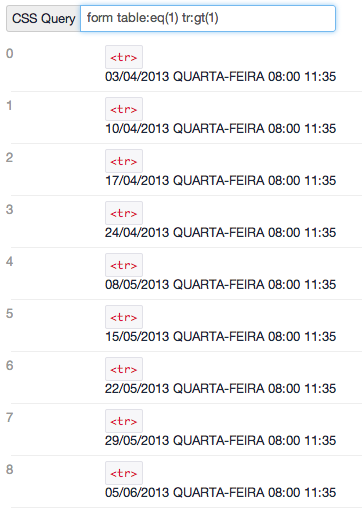
\includegraphics[scale=0.5]{imagens/listahorariossemestre.png}
     \\  Fonte: Do Autor.
\end{figure}

\newpage

A partir do retorno da expressão demonstrado na Figura 11, são aplicadas novas expressões para obter-se as informações específicas necessárias, sendo estas expressões mostradas na Tabela X.

\begin{table}[!hbt]
\centering
\caption[Extração de Informações - Expressões de Extração dos Detalhes da Disciplina]{Tabela de expressões de extração dos detalhes das disciplinas.}
\vspace{3mm}
\begin{tabular}{p{3cm}|c}\hline
\bf{Informação} & \bf{Expressão}                                 \\ \hline
Data            & td:eq(0) \\ \hline
Dia da Semana   & td:eq(1) \\ \hline
Hora            & td:eq(2) \\ \hline
Ocorreu         & b        \\ \hline
\end{tabular}
\\ Fonte: elaboração do autor.
\end{table}

Para saber se a aula já foi ministrada ou não, é validado se a informação sendo extraida está em negrito no código HTML, acrescentando-se a expressão \emph{b} a expressão original.

Desta forma, toda a extração de informações utilizando a biblioteca \emph{jsoup} é finalizada, sendo necessário agora preprar o arquivo que será enviado ao aplicativo móvel utilizando o servidor REST.

\section{Preparação dos Dados}
A preparação dos dados para o envio para a aplicação móvel é feita em conjunto com a extração dos dados da página, porém para demonstrar de forma mais simples e facilitar o entendimento este capítulo irá demonstrar apenas o layout dos arquivos gerados. 

Toda a geração dos arquivos funciona como retorno das funções de extração, sendo que o retorno ocorre em formato JSON, devido ao formato simples de representação de dados e economia da banda de dados se comparado com o formato XML, já que o JSON não possui tags de fechamento e cabeçalho nos arquivos. Não existe muitas coisas a serem explicadas sobre os arquivos gerados, pois os mesmos são de fácil leitura e entendimento, e juntamente com as informações já comentadas no item 5.2 deste trabalho causaria redundância nas informações.

\section{Servidor REST}
Após extração e preparação dos dados, resta apenas disponibilizar as informações para acesso externo. Para esta tarefa foi utilizada a classe IceBreakRestServer, que implementa um servidor REST básico que supre as necessidades deste trabalho. Foi necessária apenas uma alteração no cabeçalho HTML retornado pela classe, o qual retornava tamanhos errados, que acabavam ocasionando a perda de informações do arquivo JSON. Como não é um parâmetro obrigatório do cabeçalho do HTML, o tamanho deixou de ser enviado no mesmo, e assim o problema deixou de existir. 

Como todo serviço de rede, é necessário escutar uma porta para receber as conexões, e neste trabalho foi escolhida a porta 90 para o servidor REST, pois assim não ocasionaria um conflito com a porta 80 utilizada pelos servidores HTTP.

Como possuimos três tipos de retorno no servidor, cada um referente a um módulo do sistema acadêmico, para otimizar o envio e também otimizar a extração no lado da aplicação, foram utilizados parâmetros na URL utilizada para conectar ao servidor, sendo estes parâmetros demonstradas na tabela 12.

\begin{table}[!hbt]
\centering
\caption[Servidor REST - Parâmetros do Servidor]{Tabela com os parâmetros aceitos pelo servidor REST.}
\vspace{3mm}
\begin{tabular}{p{3cm}|p{9cm}}\hline
\textbf{Parâmetro} & \textbf{Descrição} \\ \hline
usuario            & Neste parâmetro é possível passar ao servidor tanto a matrícula do acadêmico como o seu email da Unochapecó. Parâmetro Obrigatório  \\ \hline
senha              & Neste parâmetro deve ser informada a senha do acadêmico referente a matrícula ou email informado. Parâmetro Obrigatório. \\ \hline
info               & Neste campo é passado o tipo de informação que deseja ser recebida do servidor. \\ \hline
\end{tabular}
\\ Fonte: elaboração do autor.
\end{table}

\newpage
O parâmetro \emph{info} presente na Tabela 12 merece uma atenção especial, pois o mesmo não é obrigatório. Caso o mesmo seja omitido da URL de conexão com o servidor, teremos como retorno um valor booleano informando se o login é válido. Nesta implementação do servidor, são três as possíveis opções para o parâmetro \emph{info}: materiais, notas e horarios. Cada uma das opções refere-se a um dos módulos do sistema acadêmico extraidos anteriormente.

O acesso ao servidor ocorre por meio de requisições HTTP na porta 90. Por exemplo, caso se deseje se obter as informações do material de apoio de determinado acadêmico com o nome de usuário \emph{teste} e a senha \emph{teste}, e o servidor estivesse rodando localmente na máquina utilizada para consulta, bastaria utilizar a URL \url{http://localhost:90?usuario=teste&senha=teste&info=materiais}, sendo assim o servidor encarregado de validar o login e retornar as informações corretas referentes aos materiais de apoio do acadêmico.